\subsection{Konsepter}
Etter at det ble klart hva gruppa skulle gjøre, gjennomførte vi en brainstorm om hvordan brukergrensesnittet skulle se ut.
Alle på gruppa forsøkte å tegne konsepter på grensesnittet, og her er noen av ideene som ble brukt i konseptene:
 
%TODO

\paragraph{Kart}
Oppgaven går ut på å vise data fra telemetrimodulen på bilen, og siden denne er utstyrt men en gps, er det en mulighet å vise posisjonen til bilen på et kart.

\paragraph{Riktig fart}
Ideen var et speedometer som ikke viste hastiget, men hastighet relativt til optimal hastighet. 
Siden bilen bruker mindre energi ved lavere hastighet, ønsker man å holde en så lav hastighet som mulig, men fullføre løpet innen gitt tid.
Et slikt speedometer vil da vise hvor mye man bør øke eller senke hastigheten for å komme i mål akkurat tidsnok.

\paragraph{Tid og splittid}
Konseptet bestod av en tabell med rundetider og splittider.
Splittidene listes opp horisontalt for hver runde, og rundene listes opp vertikalt.
Tidene skal kunne vises enten som brukt tid, eller differansen mellom planlagt og brukt tid.
Dette gjør det lett å sammenligne de ulike rundene, og planlegge ulike hastigheter for disse.

\paragraph{Trending av måledata}
Siden måledata hele tiden endrer seg, vil det være interessant å se hvordan dataene har endret seg over tid.

\paragraph{Bruk av farger}
Å benytte farger til måledata vil kunne gjøre det enklere for en bruker å vite betydningen av en måleverdi.

\paragraph{Skjuling av måleverdier}
Siden måledata er mest interessante når de ikke er innen normale verdier, kan disse skjules når de normale.
Dette vil gi brukeren mindre data å holde orden på.

\subsection{Vurdering}
For å vurdere disse konseptene valgte vi å ta et møte med ecomarathon teamet, siden vi manglet grunnlag for å sette opp en vurderingsmatrise. 
Vi snakket først med Jardar, og tegningen til Hans (Figur \ref{gui-concept}) falt i god smak. 
Det ble klart at tid var langt mer viktig enn fart, så hovedskjermbildet ble det avgjort skulle først og fremst inneholde rundetider og et kart over banen. 
Trending av data ble det klart burde kombineres med å holde disse skjult når disse ikke var interessante.
Ideen om å vise splittider ble etter hvert avvist av Uwe, som mente disse ville bli vanskelige å implementere. 
Et av problemene er at man ikke har nøyaktige avstander på banen, men også at man er nødt til å stoppe en gang for hver runde.

\begin{figure}[H]
\caption{GUI-konsept} 
\label{gui-concept}
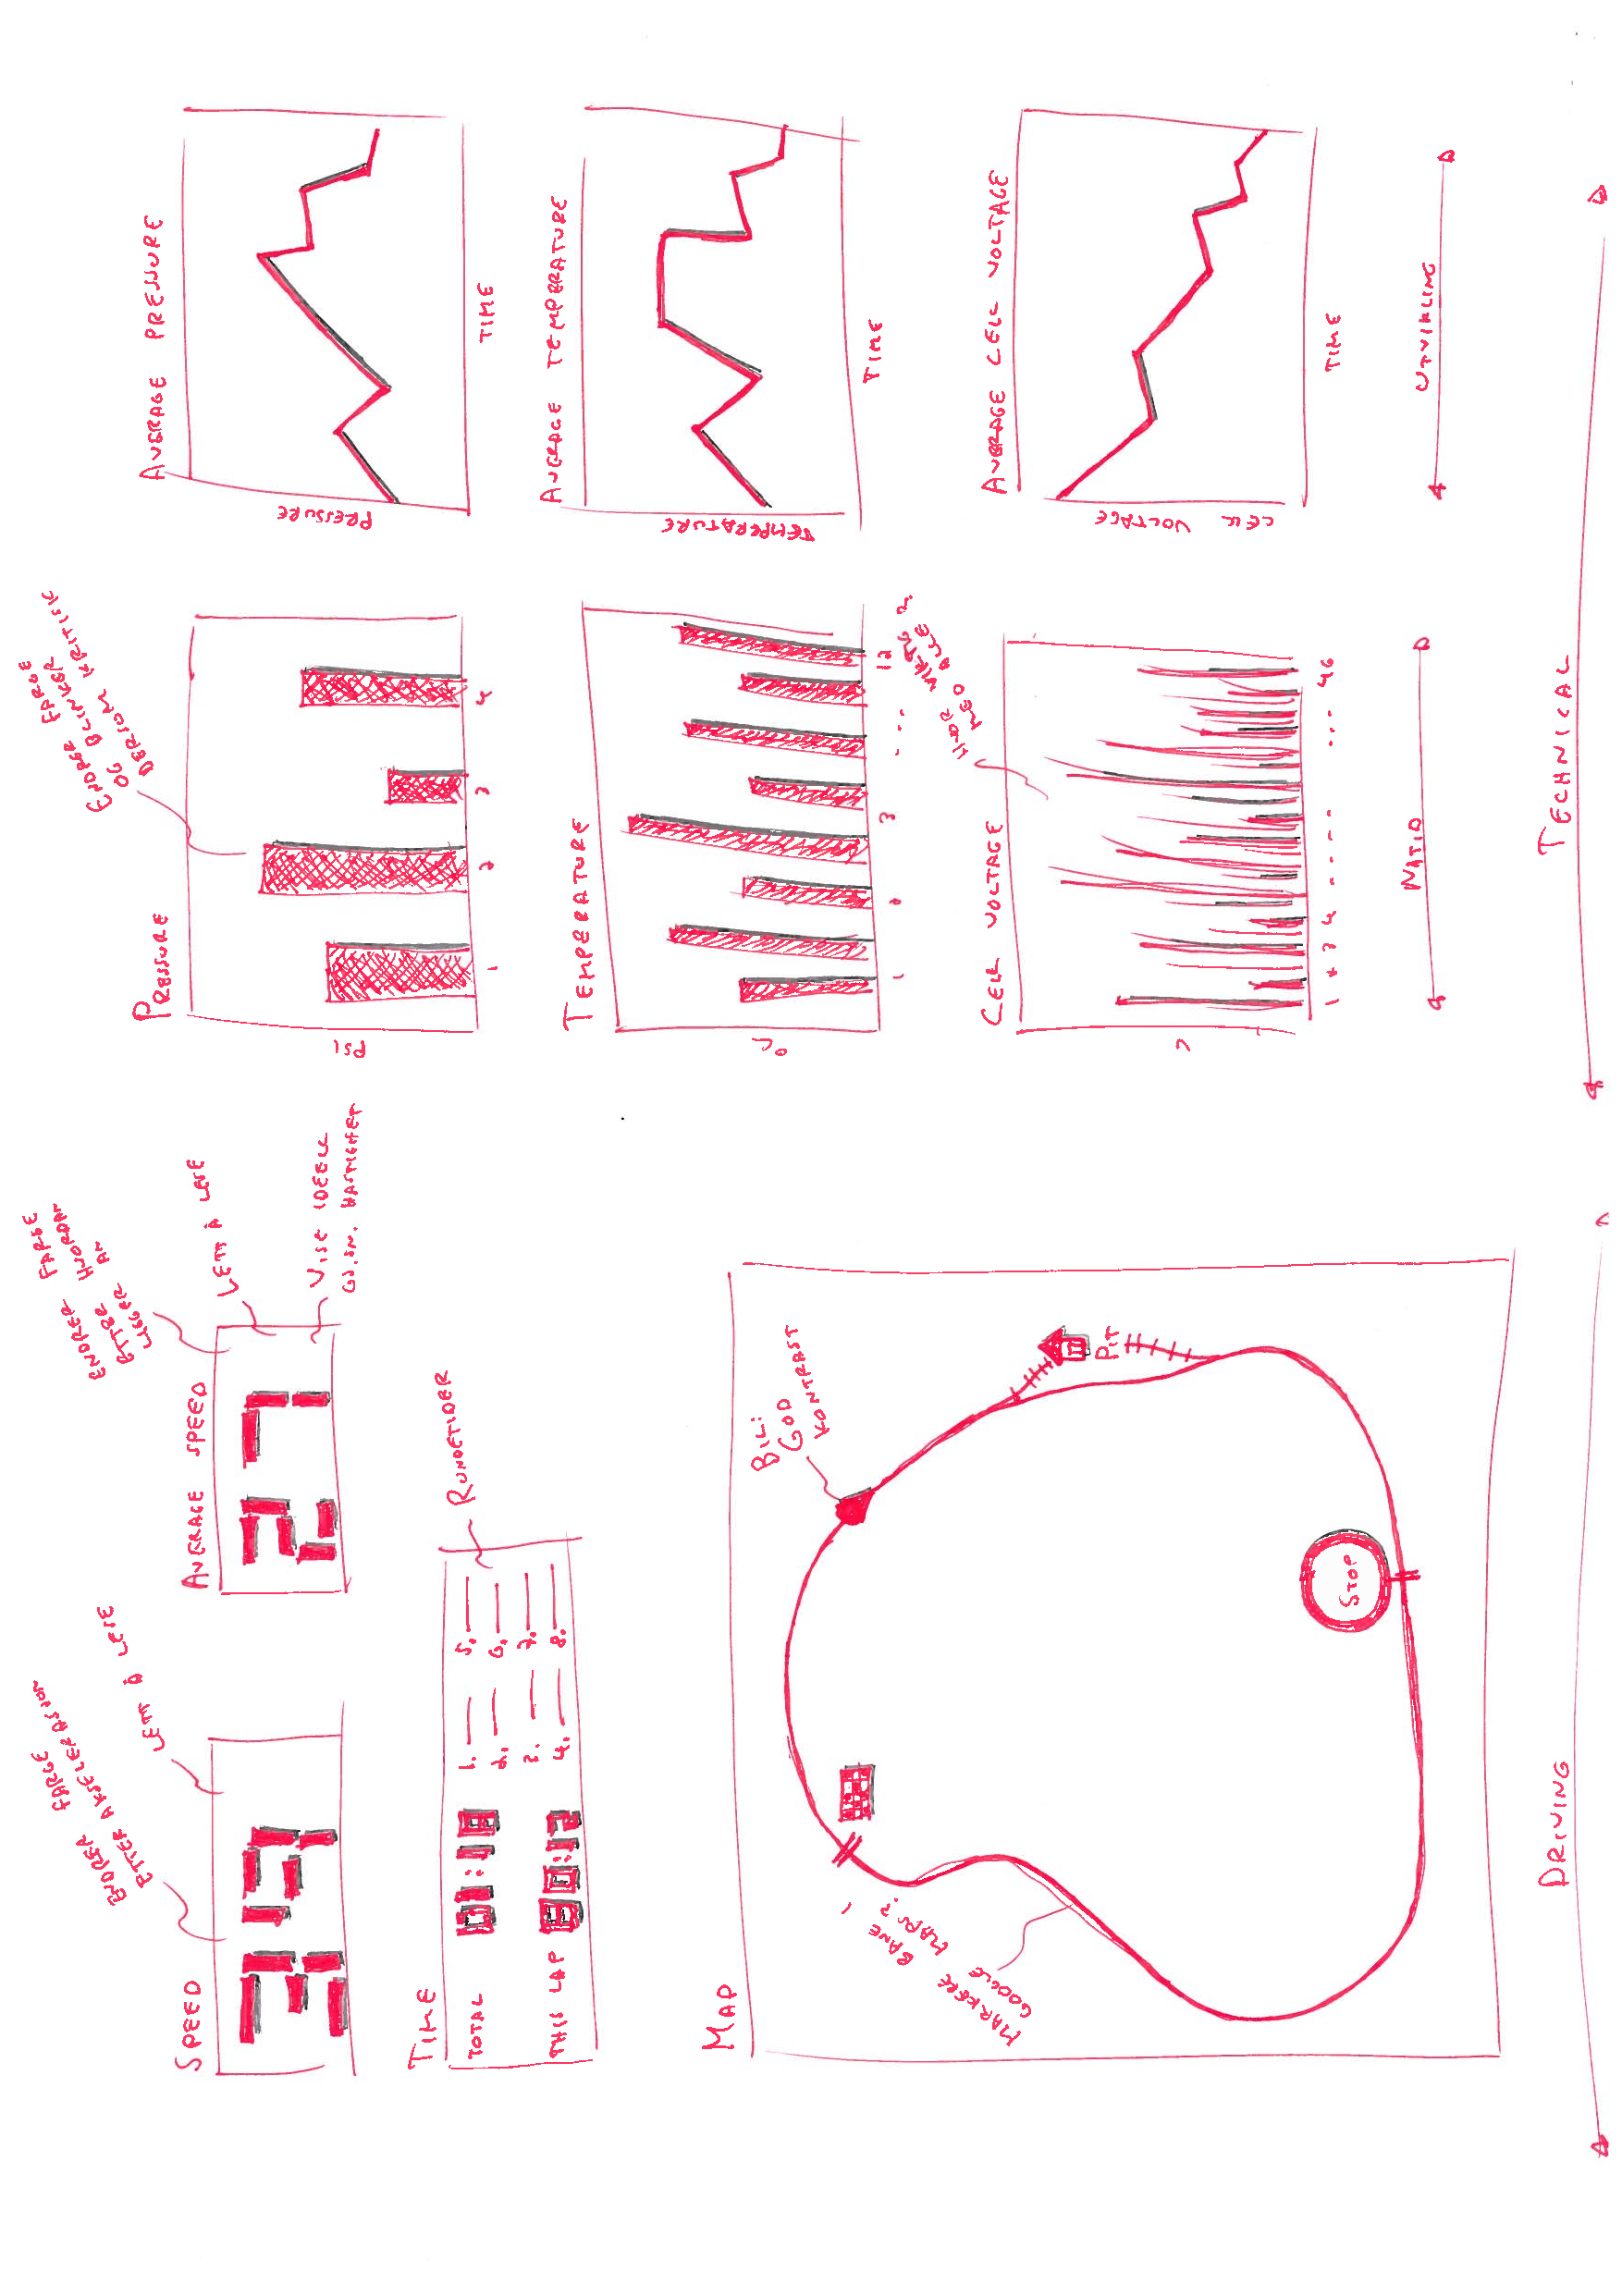
\includegraphics[width=\textwidth]{images/gui_concept_hans.pdf}
\end{figure}
